\subsubsection{\atlasC{Prospects for diboson resonance at HL- and HE-LHC}}
\contributors{R. Les, V. Cavaliere, T. Nitta, K. Terashi et al. ATLAS}
%{\bf Author(s): R. Les, V. Cavaliere, T. Nitta, K. Terashi et al. ATLAS}

%Many of searches for new heavy particles are motivated by models that aim to resolve the hierarchy problem, an unnaturally large
%difference in the strength between the electroweak and gravity forces, such as the Randall--Sundrum (RS) model with a warped extra 
%dimension or by models with composite Higgs bosons.
%Possible extensions to the SM, such as extended Higgs sectors as in the 2HDM models or extended gauge sectors as in 
%Grand Unified Theories are also motivations for new heavy particle searches.
%No clear hint of new heavy particles has been observed to date at the LHC, placing strong  constraints on the production of 
%such new particles by both ATLAS and CMS. 
Prospects are presented~\cite{ATL-PHYS-PUB-2018-022} for the search for resonances decaying to diboson ($WW$ or $WZ$, collectively called $VV$ where $V=W$ or $Z$) 
in the semileptonic channel where one $W$-boson decays leptonically and the other $W$ or $Z$-boson decays to quarks 
($\ell\nu qq$ channel). The results include sensitivity for such new resonances based on an integrated luminosity of 300 or 3000 fb$^{-1}$  
of $pp$ collisions at $\sqrt{s}$= 14 TeV using the ATLAS upgraded detector.
Searches in other semileptonic and fully hadronic decay channels are expected to have similar sensitivities at high masses, 
as observed in the ATLAS searches with Run 2 data.

While the presence of resonances is the most dramatic signal for new phenomena, they may be too heavy or broad to be clearly seen at the LHC. 
The study of the high-energy scattering between the longitudinal components of the vector bosons (vector boson scattering or VBS) is a 
perfect case to search systematically for the presence of new particles or interactions behind the breaking of the EW symmetry.  
In fact the scattering amplitude of the VBS processes, in absence of the Higgs boson, would grow indefinitely  with the \com energy, 
while it is finite if the Higgs boson is exactly the one predicted by the SM and its contributions are included. This important high-energy
behavior still needs to be tested experimentally and it will be one of the main drivers of the physics program for the HL-LHC. 
%ATLAS has recently presented results of VBS searches in the $\ssWW$ channel~\cite{ATLAS-CONF-2018-030} and $WZ$ channel~\cite{ATLAS-CONF-2018-033}  
%with $6.9\sigma$ and $5.6\sigma$ evidence respectively. 
%The existing Run-2 VBS measurements have focused on channels involving the fully leptonic boson decays 
%($W\ell\nu$ and $Z\ell\ell$)  and photons.
%The semileptonic channels, i.e., $\Vqq\Zvv$, $\Vqq\Wlv$ and $\Vqq\Zll$, can however offer some interesting
%advantages. The $\Vqq$ branching fractions are much larger than the leptonic
%branching fractions and the use of jet substructure techniques with large-radius jet reconstruction allows to 
%reconstruct and identify the $V$-boson produced in the high-$\pT$ region, which is the most sensitive to new physics effects.
The sensitivity of the ATLAS experiment to VBS in the $\ensuremath{V(q q^{\prime})} \ensuremath{W(\ell\nu)}$ final state, assuming an integrated 
luminosity of 300 or 3000 fb$^{-1}$  of $pp$ collisions at $\sqrt{s}$= 14 TeV is also presented. 
The analysis is based on event selection and classification similar to those used in the Run 1 and Run 2 ATLAS 
searches. 

%Both exotic resonance and VBS analyses use generator-level samples of the main signal and background
%processes, combined with the parameterizations of the detector performance (muon and jet reconstruction
%and selection efficiencies and momentum resolutions) expected at the HL-LHC from fully simulated
%samples. 

The prospect for resonance searches presented in this article are interpreted in the context of three different
models: a heavy vector triplet (HVT) model, a RS model and a narrow heavy scalar resonance.
The parameters of these models are chosen such that along the whole generated mass range, the resonance
widths are less than 6\% of the mass value, which is smaller than the detector resolution.
The main background sources are $W$ bosons produced in association with jets ($W$+jets), with significant contributions
from top-quark production (both  $t\bar{t}$ pair and single-top), non-resonant vector-boson pair production ($ZZ$,
$WZ$ and $WW$) and $Z$ bosons produced in association with jets ($Z$+jets). Background originating from
multi-jet processes are expected to be negligible due to the event selection requirements. 

Small- and Large-$R$ jets~(denoted by $j$ and $J$) are used in the analysis, reconstructed 
with the $\antikt$~algorithm and radius 0.4 and 1.0 respectively. It is assumed that the 
performance of a future $W/Z$-boson tagger at the HL-LHC conditions will have similar, if not better, 
performance as existing boson taggers. 
%To simulate the effect of Run-2 $W/Z$-boson tagging performance on local-calibrated topologically-clustered jets, 
%events which contain a large-$R$ jet are scaled by the expected boson tagging efficiency for the $V \to qq$ with 
%kinematics corresponding to the large-$R$ jet.
%The tagging efficiencies are calculated from fully-simulated 13~TeV MC samples as the fraction of events with a 
%large-$R$ jet passing the tagger to the number of events with large-$R$ jets within $|m(J)-m(W/Z)|<50$~GeV, 
%where $m(J)$ is the large-R jet mass. The mass cut imposed by the tagger is always smaller then the 50~GeV window applied.
%The mass window cut is applied whenever the $W/Z$-boson tagger scale factors are applied and used to incorporate 
%the shaping effect of a mass cut on the background distributions.
%Only the leading large-$R$ jet is considered for the tagging efficiency calculation.
%Separate efficiencies are calculated for each background and signal processes and applied as scale factors on the 14~TeV simulated samples.
%The $\pt$ (mass) of the large-$R$ jets is smeared using a Gaussian (Log-Normal) distribution with scale parameters derived 
%as a function of $\pt$ and $m(J)/\pt$. The large-$R$ jets in events must have $\pt>200$~GeV and |$\eta$| < 2.0.
Events are required to have exactly one lepton satisfying the selection criteria.
It is assumed that the effect of trigger thresholds is negligible for the selected leptons with $p_{T}$ studied in this note.
Events are further required to contain a hadronically-decaying $W/Z$ candidate, reconstructed either from two small-$R$ 
jets, defined as the resolved channel, or from one large-$R$ jet, designated the boosted channel.
The missing transverse energy $\met$ has to be greater than 60 GeV,
which suppresses multijet background to a negligible level.
By constraining the $\met$ + lepton system to be consistent with the $W$ mass, the $z$ component of the neutrino  momentum
can be reconstructed by solving a quadratic equation. The smallest solution is chosen and in the case where the 
solution is imaginary, only the real part is taken. \\

\textbf{Resonance search}: The presence of narrow resonances is searched for in the distribution of reconstructed diboson mass 
using the signal shapes extracted from simulation of benchmark models.
The invariant mass of the diboson system ($m(WV)$) is reconstructed from the leptonic $W$ candidate and hadronic $W/Z$ candidate, 
the latter of which is obtained from two small-$R$ jets in the resolved channel ($m(\ell\nu jj)$) or large-$R$ jet in the boosted 
channel ($m(\ell\nu J)$). 
The background shape and normalization are obtained from MC simulation with dedicated control regions to
constrain systematic uncertainties of the background modeling and normalization.
The search is divided into two orthogonal categories to identify the $\mathrm{ggF/q\bar{q}}$ and VBF production modes 
by identifying additional forward jets. If an event passes the VBF category selection for the additional forward jets 
(defined below) it is categorized as a VBF candidate event, otherwise as a $\mathrm{ggF/q\bar{q}}$ candidate event.
Events are then processed by a merged-jet selection then a two resolved-jet selection if they fail the merged selection. 
This prioritization strategy provides the optimum signal sensitivity as it favors the merged selection which contains 
less background contribution.
An example of the final distributions for the resonance search can be seen in \fig{fig:distributions_VVatlas} (left) 
for the merged $\mathrm{ggF/q\bar{q}}$ signal region. 

\textbf{Vector boson scattering search}
Experimentally, VBS is characterized by the presence of a pair of vector bosons ($W$, $Z$, or $\gamma$) and two forward jets with a large
separation in pseudorapidity and a large dijet invariant mass.
Therefore the VBS search is required to have 2 additional forward VBS-topology tagging jets in the event in addition to jets associated 
with the boson decay, similar to the resonant VBF search.
The VBS tagging jets are required to be non-$b$-tagged, in order to suppress the contribution of diagrams with a $Wtb$ vertex
(especially the electroweak $t\bar{t}$ production) in the electroweak $VVjj$ production.
Tagging jets must be in the opposite hemispheres, $\eta(j_1^{\mathrm{tag}}) \cdot \eta(j_2^{\mathrm{tag}}) < 0$,
and to have the highest dijet invariant mass among all pairs of jets remaining in the event after the $V \rightarrow jj$ jet selection greater than 400~GeV.  
%This jet prioritization scheme is the reverse of the resonant VBF scheme and offers better background rejection in the $\pt$ 
%regime of interest in the VBS search.
%After the tagging jet pair are selected, it is required that both tagging jets should have $\pt$$>$30~GeV,
%in order to suppress the contribution from pile-up, and that the invariant mass of the two tagging jets system is greater than 400~GeV .
%In the VBS search the VBS-tagging jets are selected after the signal jets and are required to be $\Delta R>1$ away from signal large-$R$ jets.
To optimize the signal sensitivity, Boosted Decision Trees (BDT) were trained on the background 
and signal MC samples in the respective regions. Further details are given in \citeref{ATL-PHYS-PUB-2018-022}%13~TeV MC.
The invariant mass distribution of the diboson pair are displayed in \fig{fig:distributions_VVatlas} (right) for the VBS search. \\

\begin{figure}[!ht]
  \begin{centering}
    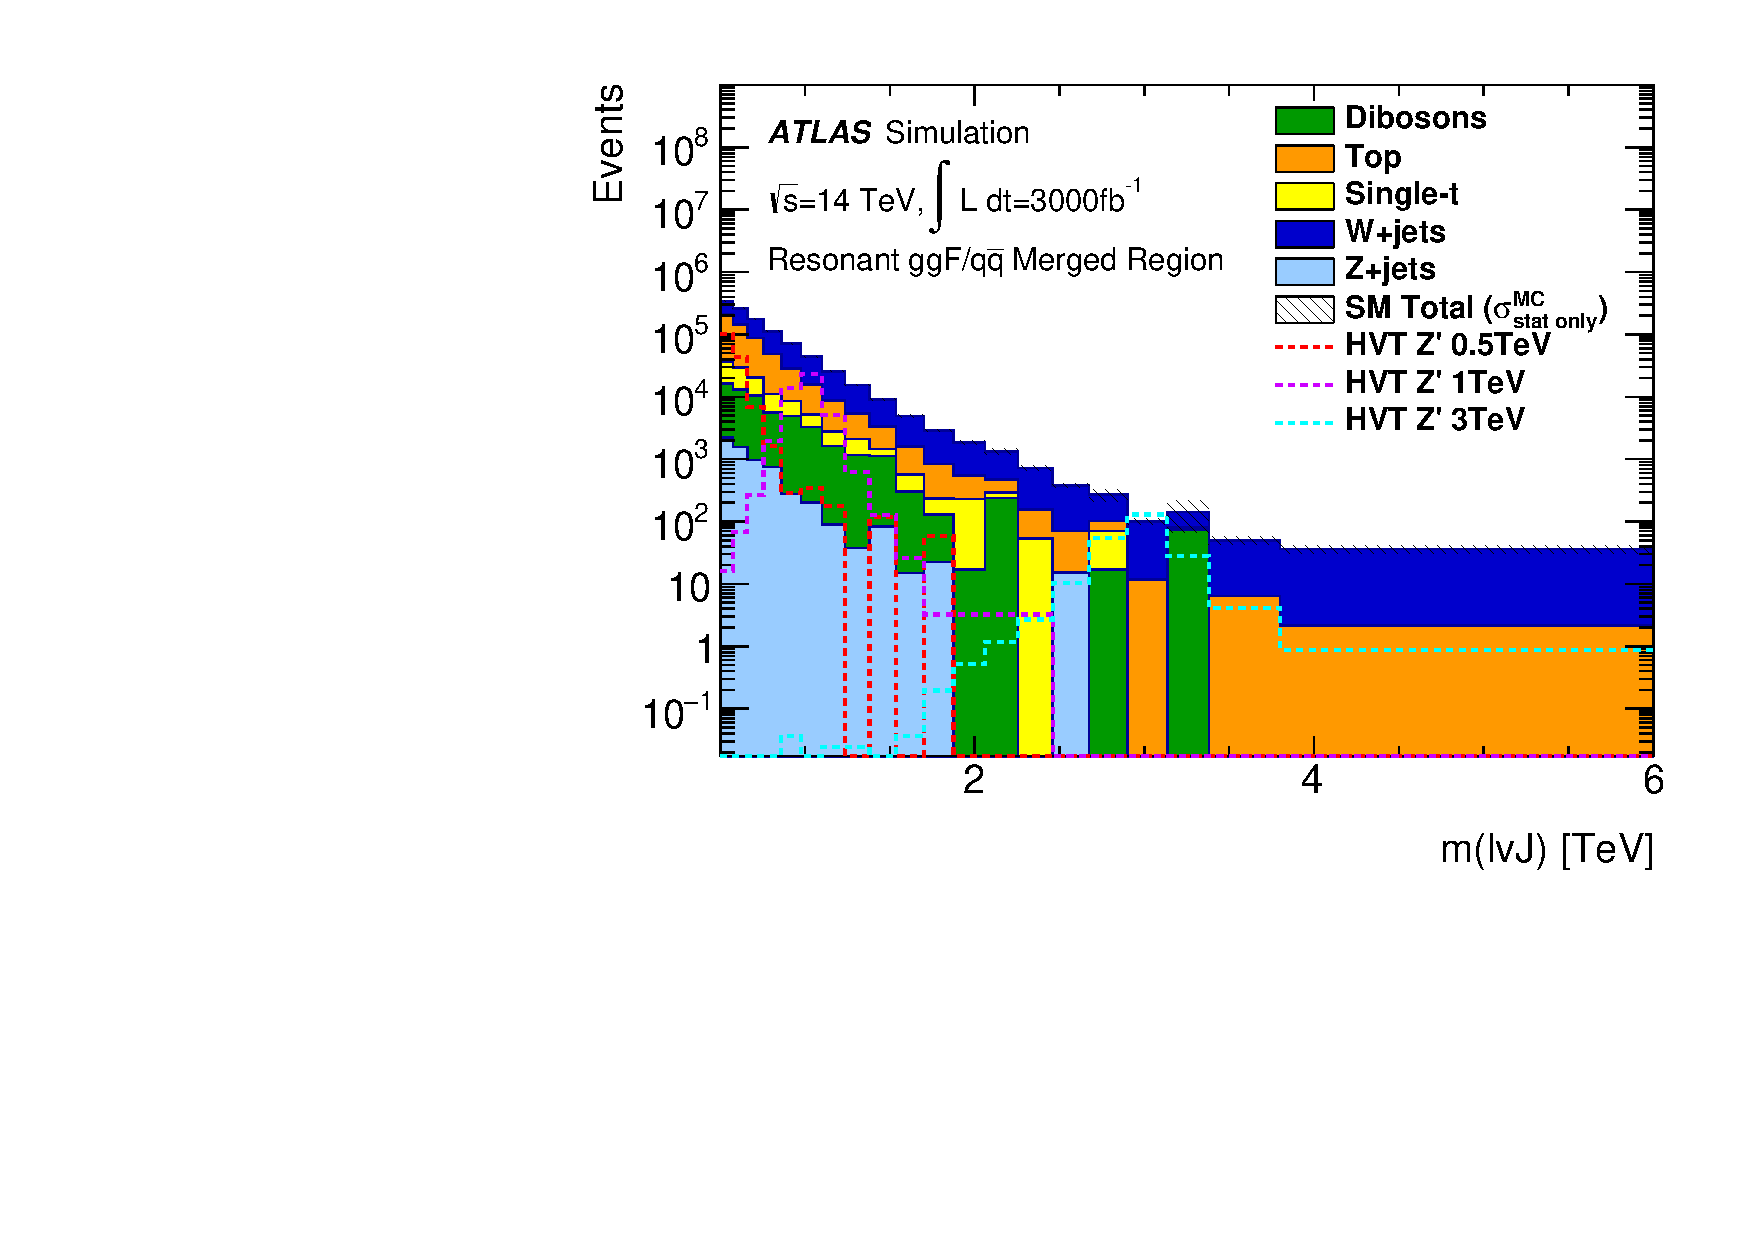
\includegraphics[width=0.45\textwidth]{\main/section7OtherSignatures/img/ResonanceMerged_lvJ_m_3000ifb_VVatlas.pdf}
    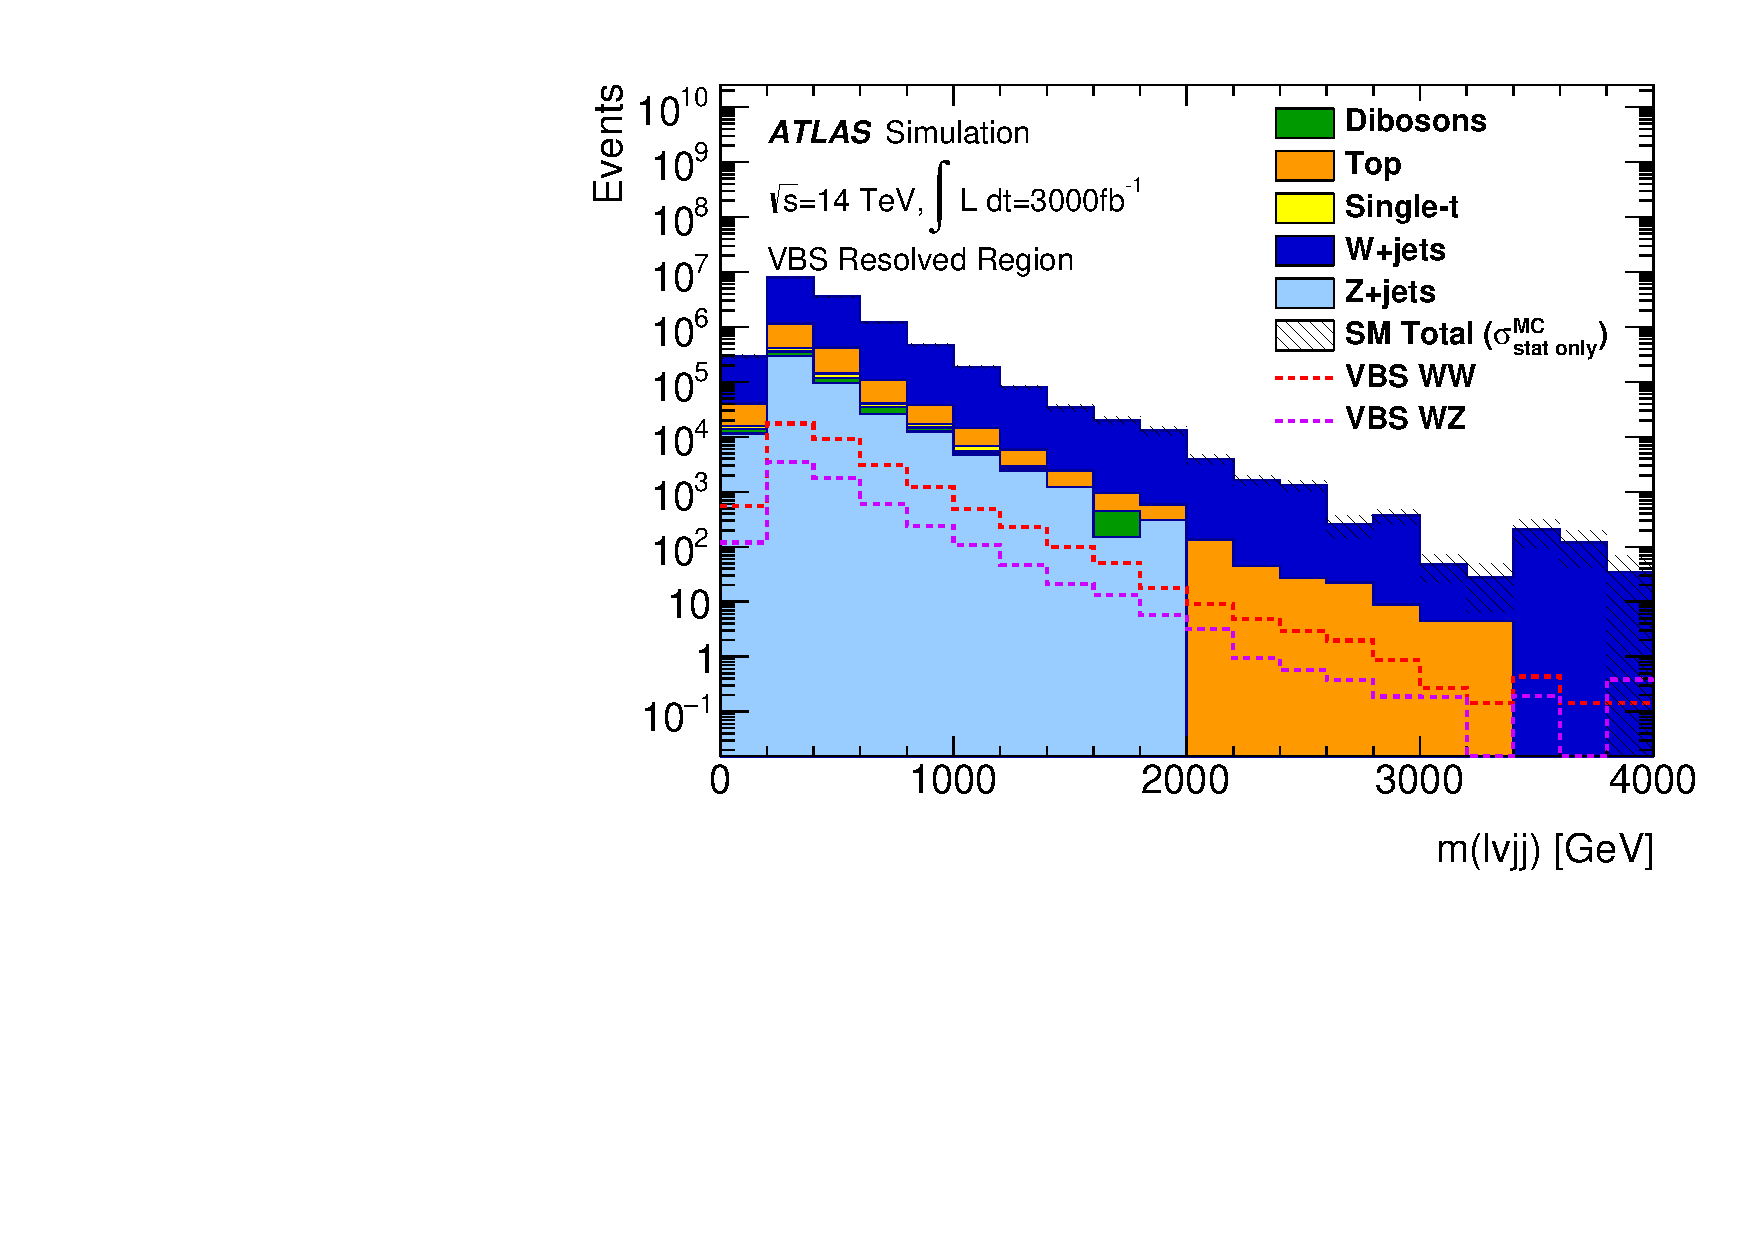
\includegraphics[width=0.45\textwidth]{\main/section7OtherSignatures/img/VBSResolved_lvjj_m_3000ifb_VVatlas.pdf}
    \caption{Left: Final $m(\ell\nu J)$ distribution in the merged signal region for the $\mathrm{ggF/q\bar{q}}$ resonance search. 
where appropriate. Right: Final signal and background distributions for the VBS search in the resolved SR for the 
the reconstructed diboson invariant mass. 
Background distributions are separated into production type. HVT and VBS signals are overlayed as dashed curves where appropriate.  }
    \label{fig:distributions_VVatlas}
  \end{centering}
\end{figure}

The results are extracted by performing a simultaneous binned maximum-likelihood fit to the $m(WV)$ distributions (BDT for the VBS search) 
in the signal regions and the $W$+jets and $t \bar{t}$ control regions. 
%The $WW$ and $WZ$ channels for the resonance search are treated individually because they partially overlap. A test statistic based on the 
%profile likelihood ratio is used to test hypothesized values of the signal cross-section, separately for each model considered. 
%The likelihood is defined as the product of the Poisson likelihoods for all signal and control regions for a given production mechanism category and channel. 
The fit includes five background contributions, corresponding to $W$+jets, $t \bar{t}$, single-top, $Z$+jets, and diboson. 
Systematic uncertainties are taken into account as constrained nuisance parameters with Gaussian or log-normal distributions. 
For each source of systematic uncertainty, the correlations across bins of $m(WV)$ distributions and between different kinematic regions, 
as well as those between signal and background, are taken into account. 
The main background modelling systematics, namely the $W$+jets and $t\bar{t}$ shape uncertainties, are constrained by the corresponding 
control regions and are treated as uncorrelated among the resolved and merged signal regions.            
%The number of bins and the bin widths in each signal region are optimized according to the expected background event distribution and detector 
%resolution. In all regions, the overflow events are included in the last bin. 
The expected upper limits are set on the signal cross section times branching ratio as a function of the signal mass.  
For the HVT $W'$ and $Z'$ the limits are estimated to be 4.3 TeV with L =300 fb$^{-1}$ and and 4.9 TeV with L =3000 fb$^{-1}$ of $pp$ collisions, 
using the same detector configuration and pileup conditions. For the Bulk graviton the expected limits are estimated as 2.8 and 3.3~TeV 
at L =300 fb$^{-1}$ and L =3000 fb$^{-1}$.
The values at L =3000 fb$^{-1}$ show an expected increase to the sensitivity of the search to the benchmark signals by $\sim$1 TeV with 
respect to existing limits in this channel in Run 2. 

Figure~\ref{fig:Limits_VVatlas} (left) shows one of the upper limit plots for the $\mathrm{ggF/q\bar{q}}$ category at L =3000 fb$^{-1}$.   
%assuming pile-up conditions of 200 additional collisions per-crossing. 
A line showing the theoretical cross section for the HVT $Z'$ decaying into $WW$ via $\mathrm{ggF/q\bar{q}}$ 
production at each mass is overlayed and indicates the mass reach of the search.
In the circumstance that HL-LHC sees an excess, the expected sensitivity can also be characterized.  
The discovery significance is defined as the luminosity required to see a $5\sigma$ effect of the signal. 
Figure~\ref{fig:Limits_VVatlas} (right) shows the expected discovery significance for the resonant search. 
The signal significance is the quadratic sum of $s/\sqrt{s+b}$, for each bin of the final discriminant distribution at that luminosity, 
$s(b)$ representing the number of signal(background) events in the bin.
In addition to the expected values, dashed curves shows the expected values for a future $W/Z$-tagger which has a 50\% increase 
in signal efficiency and a further factor of 2 in background rejection. 
These values are representative of improvements seen in a recent diboson resonance search in the fully-hadronic $VV \rightarrow qqqq$ 
analysis by using track-caloclusters as opposed to locally-calibrated topologically-clustered calorimeter jets.
Other possible improvements in $W/Z$-tagging in the HL-LHC era can originate from usage of more advanced machine-learning techniques to discriminate 
against the background contribution and better understanding of jet substructure variables with measurements at higher integrated luminosities.

\begin{figure}[!ht]
\begin{centering}
    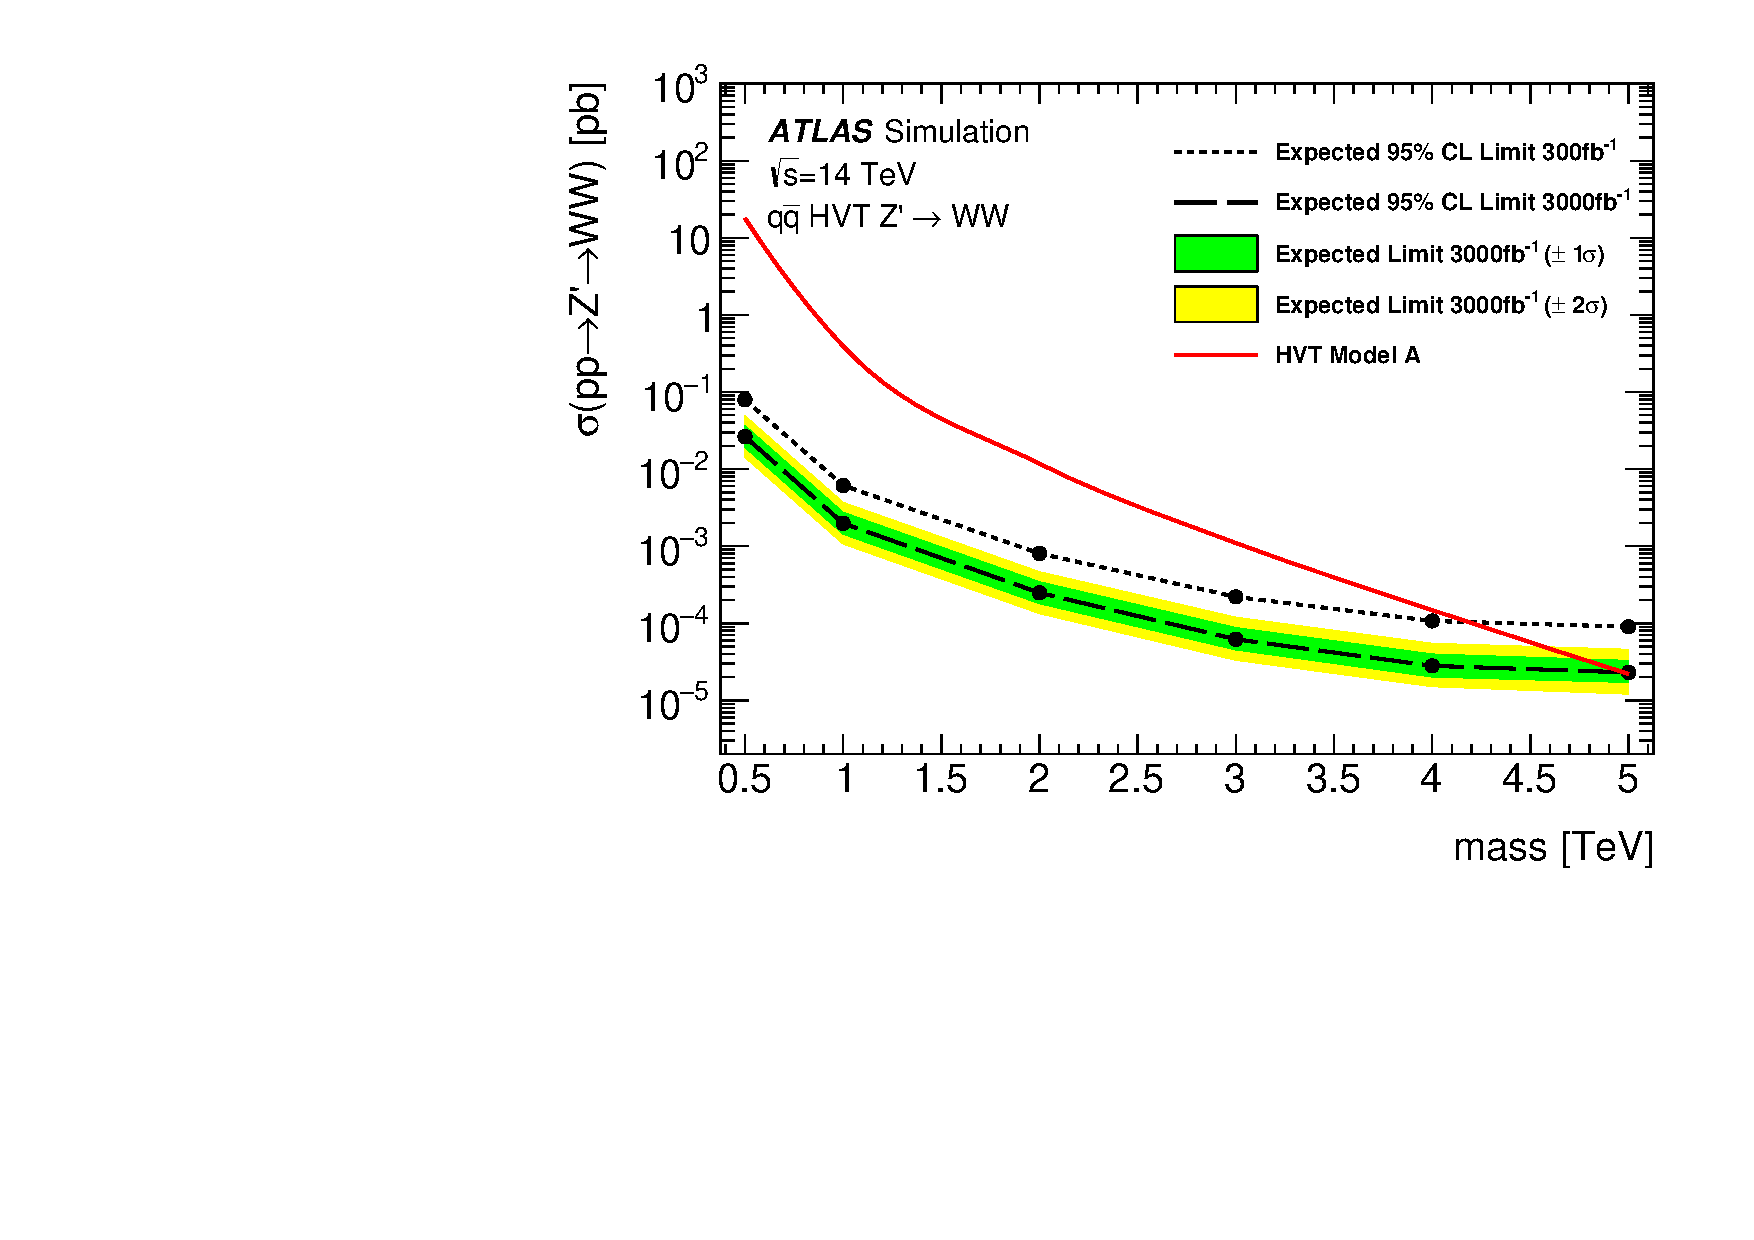
\includegraphics[width=0.45\textwidth]{\main/section7OtherSignatures/img/limits_HVTWW_VVatlas.pdf}
    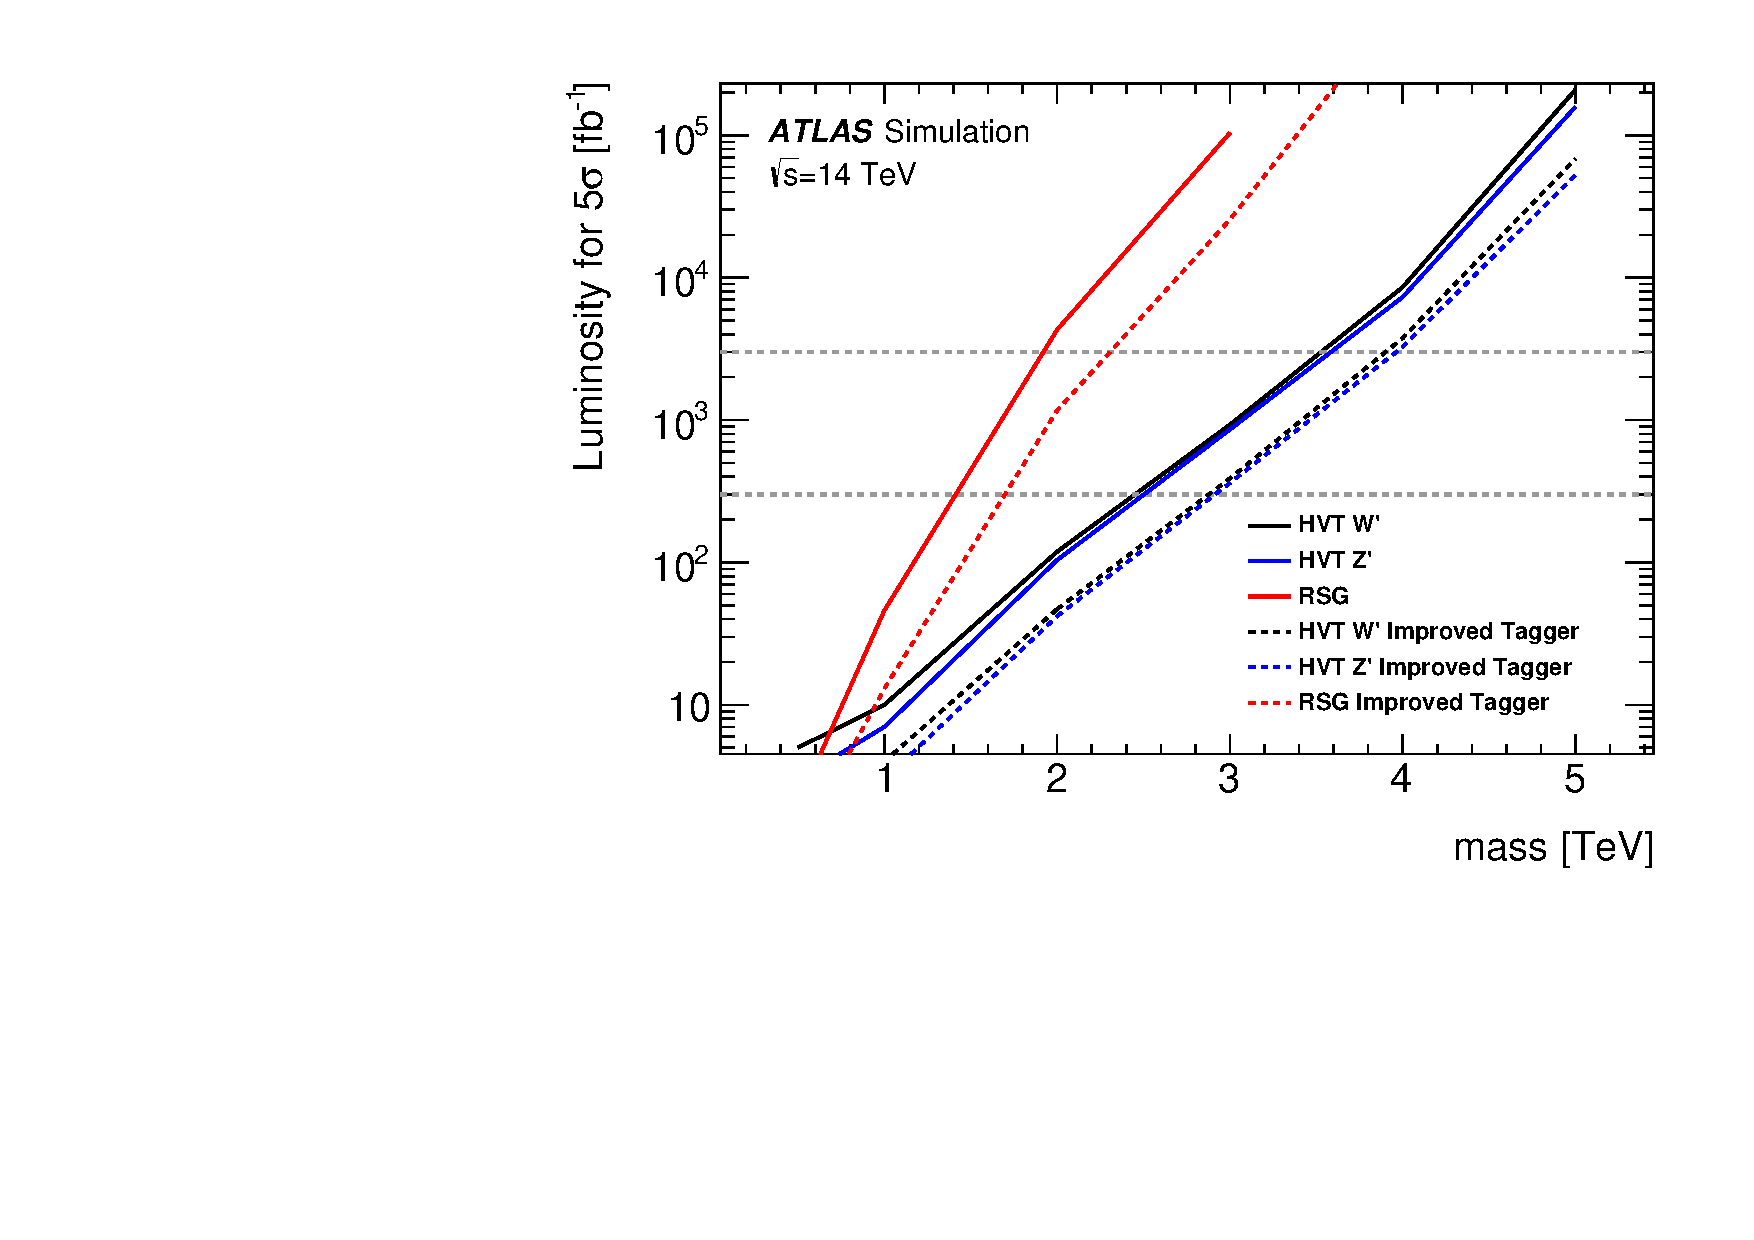
\includegraphics[width=0.45\textwidth]{\main/section7OtherSignatures/img/ResonanceDiscoverySignificance_VVatlas.pdf}
    \caption{Left: 95\%~\cl upper limit for the HVT $Z'$ via $\mathrm{ggF/q\bar{q}}$ production. Right: Expected luminosity required to observe a 5$\sigma$ signal significance for the HVT $W'$ (black), HVT $Z'$ (blue) and $G_{RS}$ (red). The solid curves shows the sensitivity using the current $W/Z$-tagger and the dashed curves for a future tagger that has a 50\% increased signal efficiency and a factor 2 increased rejection of background.}
    \label{fig:Limits_VVatlas}
\end{centering}
\end{figure}

Finally, for the VBS search, the statistical analysis is done on the signal strength of the SM VBS~($WW/WZ \rightarrow \ell\nu qq$) processes.
The expected significance for the SM VBS process is 5.7$\sigma$ at 300 fb$^{-1}$. The expected cross-section uncertainties are 18\% at  300 fb$^{-1}$ 
and 6.5\% at 3000 fb$^{-1}$. The effects of unfolding were not considered for the cross-section estimates.
 
\textbf{Resonance search at HE-LHC}

The prospect analysis at HE-LHC  mimics the analysis at HL-LHC but the Delphes simulation is used. 
Results are  interpreted in the context of the  heavy vector triplet (HVT) model~\cite{HVT,Pappadopulo:2014qza}.
The major backgrounds $W$+jets and $t\bar{t}$ production are simulated with \textsc{Madgraph} and \textsc{aMC@NLO} respectively, interfaced with Pythia. $Z$+jets, single top and diboson contribution are not simulated and are expected to contribute at most 10\% to the total background.

The analysis sensitivities to the resonance signals are extracted by performing a simultaneous binned maximum-likelihood fit to the $m_{WW}$ distributions as in the HL-LHC in the signal regions and the $W$+jets and $t \bar{t}$ control regions. The signal region and control regions are defined in the same way.

The expected upper limits set on the signal cross section times branching ratio as a function of the signal mass are shown in \fig{fig:Limits} at 27~TeV and compared to the limits obtained for HL-LHC . 
Based on the $Z'$ production cross section from the HVT signal model the exclusion mass reach is extracted to be 9 and 11~TeV for integrated luminosities of 3 and 15~ab$^{-1}$ at 27~TeV, using 
Delphes simulation of a potential detector configuration under no pileup condition.

\begin{figure}
\centering
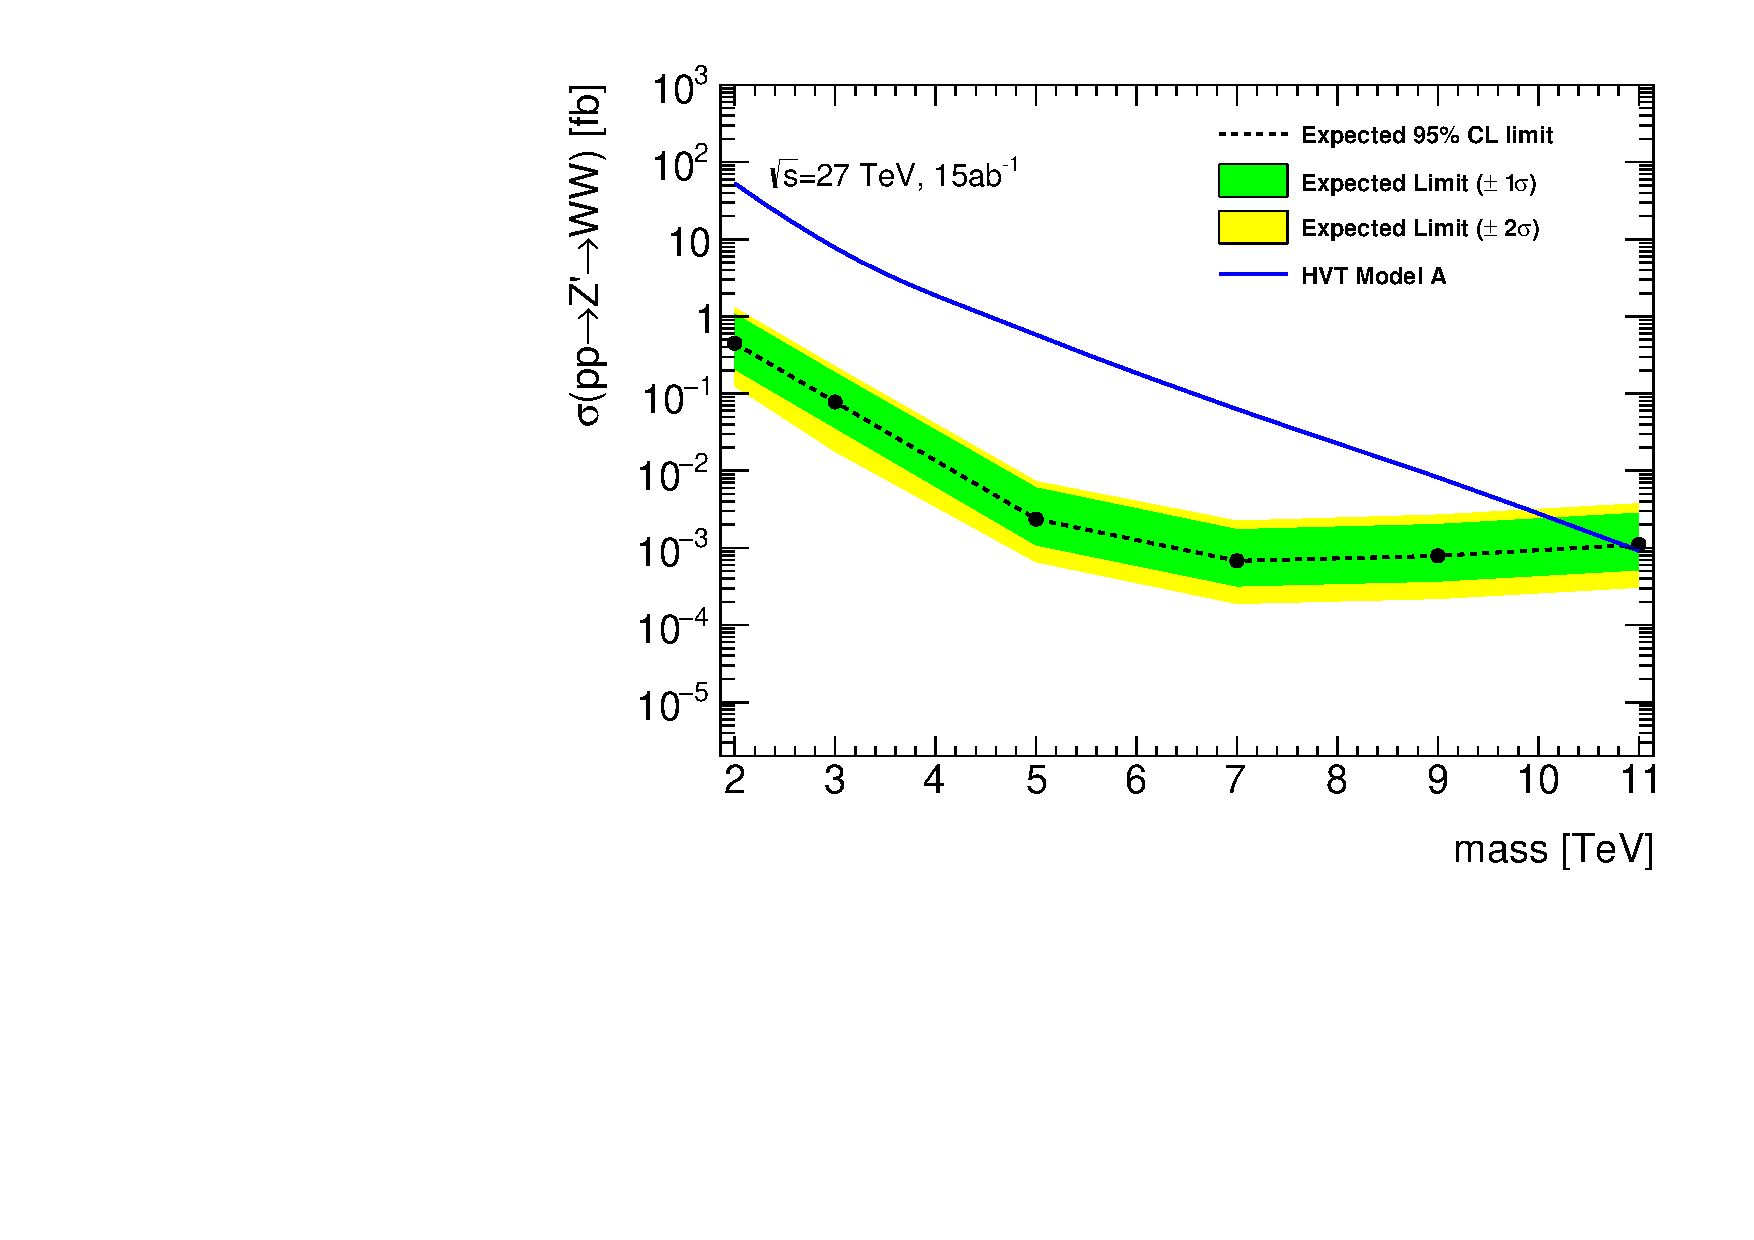
\includegraphics[width=0.45\textwidth]{\main/section7OtherSignatures/img/limits_res_atlas_helhc.pdf}
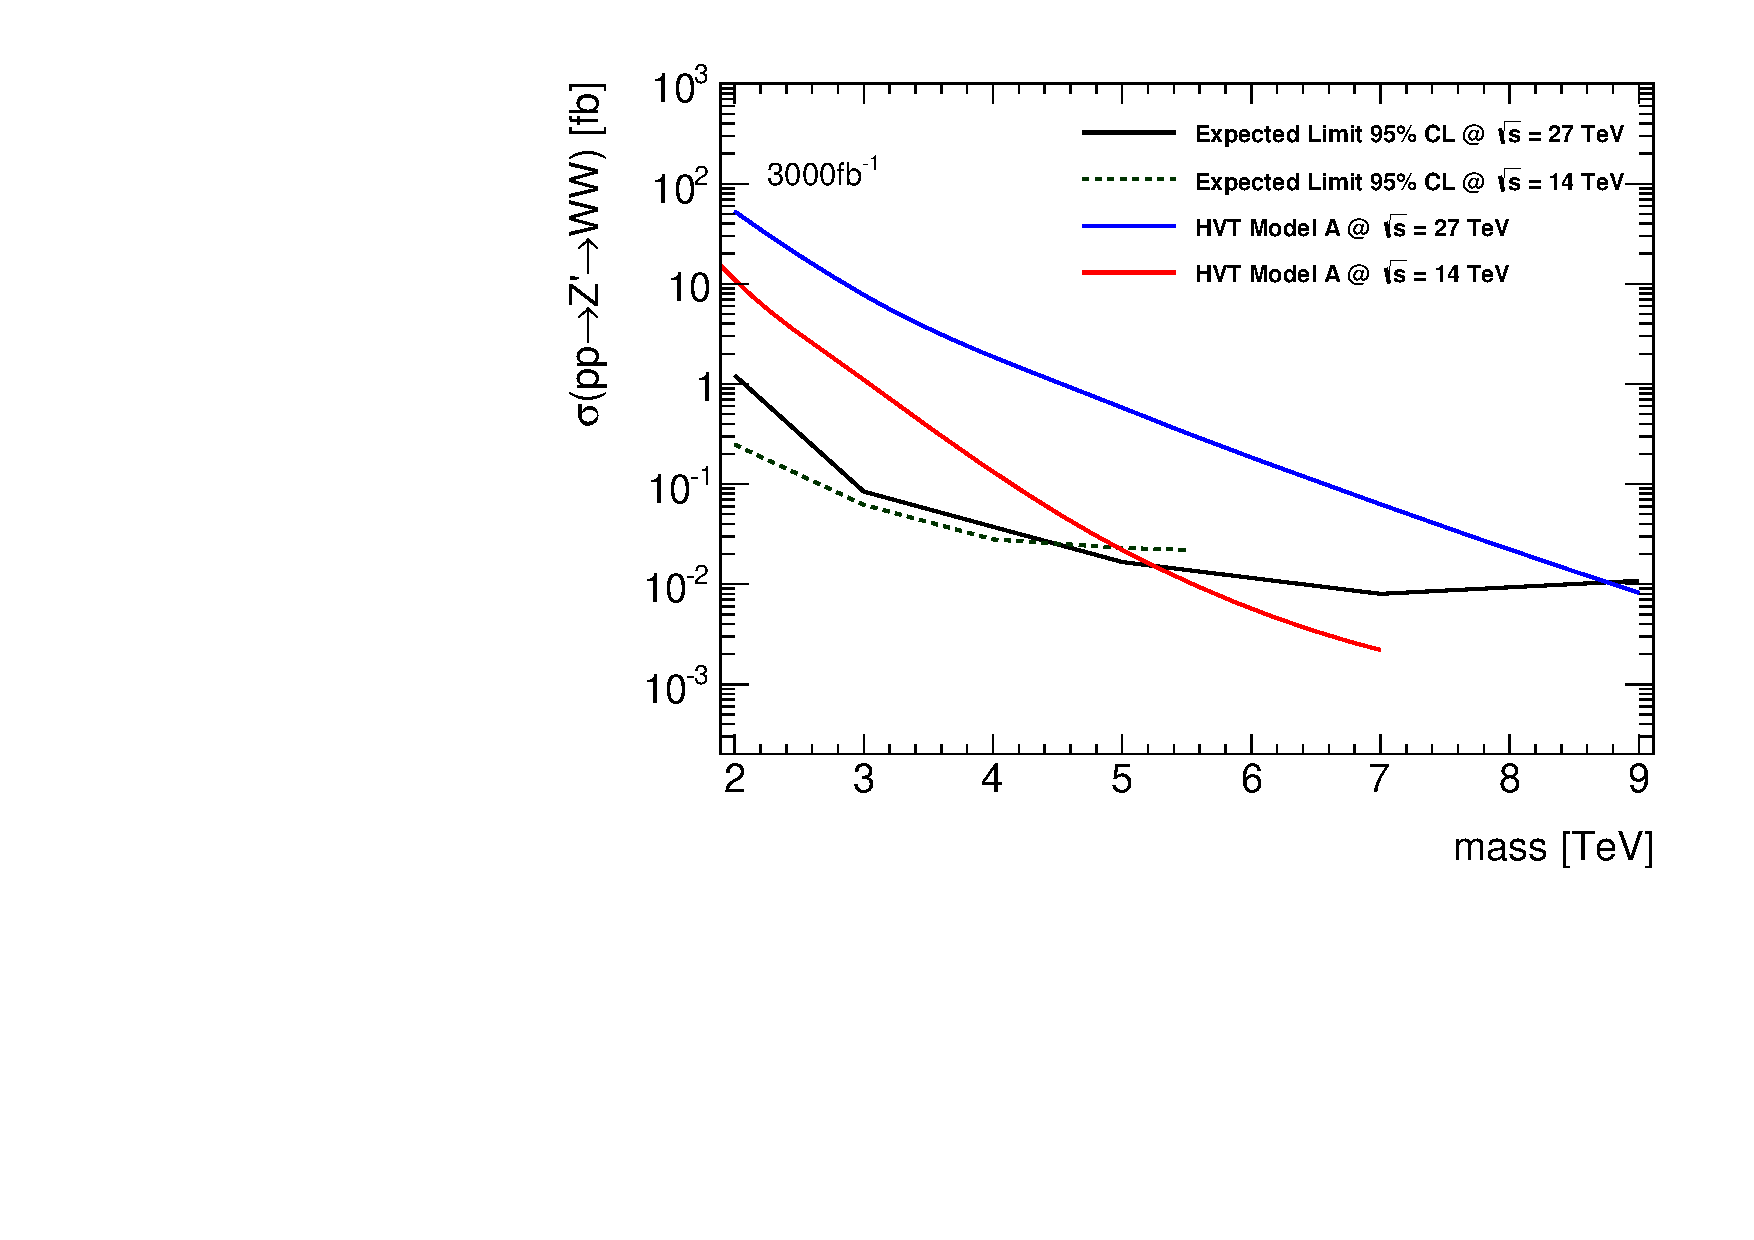
\includegraphics[width=0.45\textwidth]{\main/section7OtherSignatures/img/Comparisonlimits_res_atlas_helhc.pdf}
\caption{95\%~\cl upper limit for the HVT $Z'$  via $\mathrm{ggF/q\bar{q}}$ production.}
\label{fig:Limits}
\end{figure} 








